\pdfmapfile{+univers}%
\pdfmapfile{+dinbold}%
\documentclass[ngerman]{beamer}
\usepackage[utf8]{inputenc}
\usepackage[T1]{fontenc}
\usepackage[ngerman]{babel}
\usepackage{graphicx}
\usepackage{svg}
\usetheme[pagenum,nosectionnum,noheader,transition=push,headline=light]{tud}
\begin{document}
\title{FoodShip Group Update}
\subtitle{FoodShip, a foodsharing App}
\author{Sönke Huster \& Hannes Hilbert}
\date{\today}

\maketitle

  %  \frame{\frametitle{Inhaltsverzeichnis}\tableofcontents}

\section{Scenario}
\subsection{App Idea}
\frame{\frametitle{App Idea}
    \begin{itemize}
        \item Get to know your nameless neighbourhood through shared, spontaneous dinners
        \item App proposes having dinner with users nearby and a recipe based on the groups fridge content
    \end{itemize}
}
\section{App Development}
\subsection{Technologies}
\frame{\frametitle{Technologies}
\begin{itemize}
\item  Mobile Application:
\begin{itemize}
  \item Android application (Java)
  \item Location tracking
\end{itemize}
\item Server:
  \begin{itemize}
    \item Server Application with RESTful API
  \end{itemize}
\end{itemize}
}

\subsection{Architecture}
\frame{\frametitle{Architecture}
\begin{figure}
  \centering
  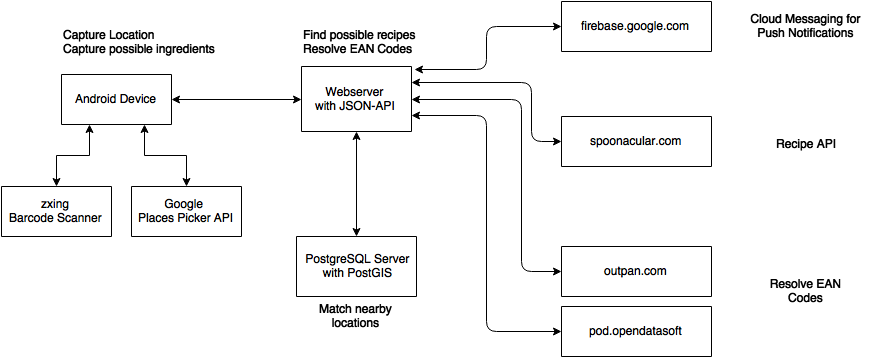
\includegraphics[width=0.9\textwidth,height=\textheight,keepaspectratio]{../diagrams/architecture_2.png}
\end{figure}
}

\section{Challenges}
\frame{\frametitle{Challenges}

\begin{itemize}
\item  Connectivity challenge
\begin{itemize}
    \item Good looking recipes independent from connection type
\end{itemize}
\item  Offline Challenge
\begin{itemize}
    \item Keep recipes and dinner information while offline
    \item Add food while offline
\end{itemize}
\item  Energy Challenge
\begin{itemize}
    \item Keep invitations up to date
    \item Know the rough location
\end{itemize}
\end{itemize}
}
\subsection{Workplan}
\frame{\frametitle{Workplan}
\begin{itemize}
  \item 16.12.2016 Second presentation
  \item 13.01.2016 End of implementation
  \item 27.01.2016 Third presentation
\end{itemize}
}
\end{document}
